\documentclass[10pt]{article}

\usepackage[utf8]{inputenc}
\usepackage[T1]{fontenc}
\usepackage{lmodern}
\usepackage{amsmath,amssymb,amsthm}
\usepackage{array,booktabs}
\usepackage[table]{xcolor}
\usepackage{enumitem}
\usepackage{geometry}
\usepackage{hyperref}
\usepackage{algpseudocode}
\usepackage{pgfplots}
\pgfplotsset{compat=1.18}
\usepackage[ruled, vlined, algoruled]{algorithm2e} % Options for styling
\usepackage{tikz}
\geometry{top=0.65in,bottom=0.65in,left=0.7in,right=0.7in}
\hypersetup{
  colorlinks=true,
  linkcolor=blue!60!black,
  urlcolor=cyan!50!black,
  linktoc=all
}
\setlist{nosep,leftmargin=*}
\renewcommand{\arraystretch}{1.2}
\newcolumntype{P}[1]{>{\raggedright\arraybackslash}p{#1}}

\theoremstyle{definition}
\newtheorem{definition}{Definition}[section]
\newtheorem{theorem}[definition]{Theorem}
\newtheorem{lemma}[definition]{Lemma}
\newtheorem{remark}[definition]{Remark}

\newcommand{\OPT}{\operatorname{OPT}}
\newcommand{\ALG}{\operatorname{ALG}}
\newcommand{\poly}{\operatorname{poly}}
\newcommand{\YES}{\textsc{Yes}}
\newcommand{\NO}{\textsc{No}}
\newcommand{\NP}{\mathsf{NP}}
\newcommand{\coNP}{\mathsf{coNP}}
\newcommand{\PTIME}{\mathsf{P}}
\newcommand{\NPC}{\mathsf{NP\text{-}complete}}

% Colours used to separate the three layers of approximation proofs.
\definecolor{algblue}{RGB}{0,82,155}
\definecolor{optred}{RGB}{180,45,45}
\definecolor{bridgepurple}{RGB}{105,55,145}

\title{Course Session Selection}
\author{}
\date{}

\begin{document}

\maketitle
\tableofcontents
\newpage

\section{Mod selection}
\subsection{Formal decision problem}

\begin{definition}[\textsc{Course-Session-Selection}]
An instance specifies a finite set of courses
$\mathcal{C}=\{c_1,\ldots,c_N\}$. Course $c_i$ has $m_i$ session types
(such as lectures and tutorials). For each type $t\in\{1,\ldots,m_i\}$,
there are $n_{i,t}$ candidate sessions, represented by intervals
\[
  I_{i,t,k}=[s_{i,t,k},e_{i,t,k}],
  \qquad k\in\{1,\ldots,n_{i,t}\},
\]
where $s_{i,t,k}<e_{i,t,k}$ are rational numbers encoded in binary.

The question is whether there exists a selection function
\[
  \sigma:\{(i,t):1\leq i\leq N,\ 1\leq t\leq m_i\}
  \longrightarrow \mathbb{Z}_{>0}
\]
such that
\begin{enumerate}[label=(\roman*)]
  \item $1\leq\sigma(i,t)\leq n_{i,t}$ for every $(i,t)$;
  \item all selected intervals are pairwise disjoint: for any
  $(i,t)\neq(j,u)$,
  \[
    I_{i,t,\sigma(i,t)}\cap I_{j,u,\sigma(j,u)}=\varnothing.
  \]
\end{enumerate}
Thus exactly one session is selected for every type of every course,
and no two selected sessions clash, including sessions of the same course.
\end{definition}

\begin{remark}[Non-overlap and endpoints]
The non-overlap requirement is essential: without it, the answer is
\YES{} exactly when every session type has at least one candidate.
For the closed intervals above, non-overlap means
\[
  e_{i,t,\sigma(i,t)}<s_{j,u,\sigma(j,u)}
  \quad\text{or}\quad
  e_{j,u,\sigma(j,u)}<s_{i,t,\sigma(i,t)}.
\]
If back-to-back sessions are allowed, use half-open intervals $[s,e)$
and replace $<$ by $\leq$. The reduction below works under either convention,
since intervals intended to be disjoint have positive gaps.
\end{remark}

\subsection{Membership in \texorpdfstring{$\NP$}{NP}}

A certificate lists one candidate index $\sigma(i,t)$ for each course--type
pair. Verify that every index is valid and that every pair of selected
intervals is disjoint. With $G=\sum_i m_i$ required types, this uses
$O(G^2)$ endpoint comparisons. Each comparison has polynomial bit complexity,
so the certificate can be verified in polynomial time. Therefore,
$\textsc{Course-Session-Selection}\in\NP$.

\subsection{A direct reduction from SAT}

We use SAT in conjunctive normal form (\textsc{CNF-SAT}) as the source
problem. The construction also applies directly to \textsc{3-SAT}.
Let
\[
  \varphi=\bigwedge_{j=1}^{p}D_j,
  \qquad D_j=(\ell_{j,1}\lor\cdots\lor\ell_{j,d_j}),
\]
be a formula over variables $x_1,\ldots,x_q$, where each literal is
$x_i$ or $\neg x_i$. Let $L=\sum_{j=1}^{p}d_j$ be the total number
of literal occurrences. Give every occurrence a distinct index
$a\in\{1,\ldots,L\}$, even when a literal is repeated.
If a clause is empty, the formula is unsatisfiable; map it to a fixed
\NO{} instance consisting of two courses, each with one type and the
single candidate interval $[0,1]$. Henceforth, every clause is nonempty.

\paragraph{Idea.}
Create one course for each variable and one course for each clause,
all with exactly one session type. A variable course chooses between
two long intervals, $T_i$ and $F_i$, encoding its truth value.
A clause course chooses one short interval for one of its literals.
Place that short interval inside the variable interval corresponding
to the assignment that makes the literal \emph{false}. Consequently,
a clause can choose a literal precisely when that literal is true
under the selected variable assignment.

\begin{center}
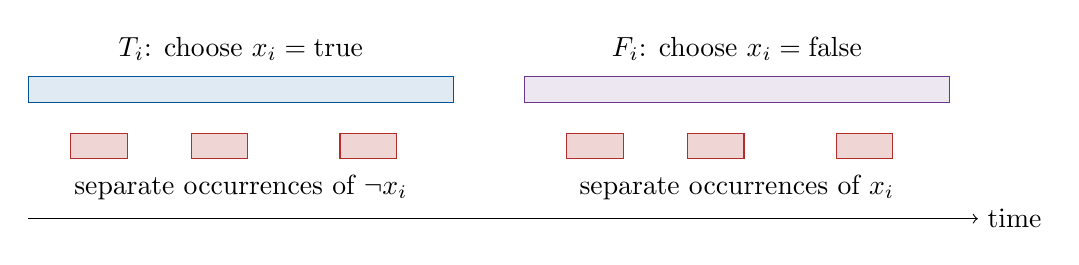
\begin{tikzpicture}[x=0.9cm,y=0.8cm]
  \draw[fill=algblue!12,draw=algblue] (0,1) rectangle (6,1.4);
  \draw[fill=bridgepurple!12,draw=bridgepurple] (7,1) rectangle (13,1.4);
  \node at (3,1.85) {$T_i$: choose $x_i=\mathrm{true}$};
  \node at (10,1.85) {$F_i$: choose $x_i=\mathrm{false}$};
  \draw[fill=optred!20,draw=optred] (0.6,0.1) rectangle (1.4,0.5);
  \draw[fill=optred!20,draw=optred] (2.3,0.1) rectangle (3.1,0.5);
  \draw[fill=optred!20,draw=optred] (4.4,0.1) rectangle (5.2,0.5);
  \draw[fill=optred!20,draw=optred] (7.6,0.1) rectangle (8.4,0.5);
  \draw[fill=optred!20,draw=optred] (9.3,0.1) rectangle (10.1,0.5);
  \draw[fill=optred!20,draw=optred] (11.4,0.1) rectangle (12.2,0.5);
  \node at (3,-0.35) {separate occurrences of $\neg x_i$};
  \node at (10,-0.35) {separate occurrences of $x_i$};
  \draw[->] (0,-0.85) -- (13.4,-0.85) node[right] {time};
\end{tikzpicture}

\small Schematic for one variable. Vertical position only separates
the drawings; overlap is determined by their horizontal time intervals.
\end{center}

\paragraph{Variable courses.}
Set $B=3L+3$ and $b_i=2(i-1)B$. For each variable $x_i$, create
a course $v_i$ with one session type and exactly two candidates:
\[
  T_i=[b_i,b_i+B-1],
  \qquad
  F_i=[b_i+B,b_i+2B-1].
\]
Selecting $T_i$ represents setting $x_i=\mathrm{true}$; selecting
$F_i$ represents setting $x_i=\mathrm{false}$.
All $2q$ variable intervals are pairwise disjoint. Although $T_i$
and $F_i$ do not clash, the requirement to select exactly one session
from their common type forces a single truth value for $x_i$.

\paragraph{Clause courses.}
For each clause $D_j$, create a course $w_j$ with one session type and
$d_j$ candidates, one for each literal occurrence in $D_j$.
For an occurrence with global index $a$, define its interval by
\[
  J_a=
  \begin{cases}
    [b_i+B+3a-2,\ b_i+B+3a-1], & \text{if the occurrence is }x_i,\\[2pt]
    [b_i+3a-2,\ b_i+3a-1], & \text{if the occurrence is }\neg x_i.
  \end{cases}
\]
Since $1\leq a\leq L$, a positive occurrence lies strictly inside
$F_i$, and a negative occurrence lies strictly inside $T_i$.
Different occurrences in the same variable interval occupy separate
slots with positive gaps; occurrences in different variable intervals
are also disjoint. Thus \emph{all clause-candidate intervals are
pairwise disjoint}, even across different clauses.

The only possible conflicts are therefore
\[
  \begin{array}{c|c|c}
    \text{literal represented by }J_a & \text{interval conflicting with }J_a
      & \text{assignment making the literal false} \\
    \hline
    x_i & F_i & x_i=\mathrm{false} \\
    \neg x_i & T_i & x_i=\mathrm{true}
  \end{array}
\]
The constructed course set is
$\mathcal{C}_\varphi=\{v_1,\ldots,v_q,w_1,\ldots,w_p\}$.

\paragraph{Polynomial size.}
There are $q+p$ courses, one type per course, and $2q+L$ candidate
sessions. All endpoints are nonnegative integers smaller than
$2qB=O(q(L+1))$, so they have $O(\log((q+1)(L+1)))$ bits.
The construction is computable in polynomial time.

\subsection{Correctness and NP-completeness}

\begin{lemma}
The formula $\varphi$ is satisfiable if and only if the constructed
\textsc{Course-Session-Selection} instance has a feasible selection.
\end{lemma}

\begin{proof}
\noindent\textbf{($\Rightarrow$)} Suppose $\varphi$ has a satisfying
assignment. For every variable course $v_i$, select $T_i$ if $x_i$ is
true and $F_i$ otherwise. These selected variable intervals are
pairwise disjoint.

Every clause has a true literal. For each clause course, select the
candidate $J_a$ of one such literal. If the literal is $x_i$, then
$J_a$ lies inside the unselected interval $F_i$; if it is $\neg x_i$,
then $J_a$ lies inside the unselected interval $T_i$. In either case,
$J_a$ is disjoint from every selected variable interval. All selected
clause intervals are also pairwise disjoint by construction. Thus we
obtain exactly one session per course type with no conflicts.

\medskip
\noindent\textbf{($\Leftarrow$)} Suppose the constructed instance has
a feasible selection. Each variable course selects exactly one of
$T_i,F_i$. Set $x_i$ to true exactly when $T_i$ is selected.

Consider any clause course $w_j$ and its selected interval $J_a$.
If $J_a$ represents $x_i$, it overlaps $F_i$, so feasibility forbids
selecting $F_i$. Therefore $T_i$ is selected and $x_i$ is true.
If $J_a$ represents $\neg x_i$, the same argument forbids $T_i$,
so $F_i$ is selected and $\neg x_i$ is true. Hence every clause
has a true literal, and the extracted assignment satisfies $\varphi$.
\end{proof}

\begin{theorem}
\textsc{Course-Session-Selection} is NP-complete, even when every
course has exactly one session type, every type has at most three
candidate sessions, and all endpoints are nonnegative integers.
\end{theorem}

\begin{proof}
The problem belongs to $\NP$ as shown above. The polynomial-time
construction and the correctness lemma give the direct reduction
\[
  \textsc{CNF-SAT}\leq_p\textsc{Course-Session-Selection}.
\]
This proves NP-hardness. For the stated restriction, apply the same
construction to \textsc{3-SAT}: each variable type has two candidates
and each clause type has at most three. Thus the restricted problem,
and consequently the general problem, is NP-complete.
\end{proof}


\end{document}
